\documentclass[10pt]{beamer}
\usepackage[T1,T2A]{fontenc}
\usepackage[utf8]{inputenc}
\usepackage{hyperref}
\hypersetup{unicode=true}
\usepackage{fontawesome}
\usepackage{graphicx}
\usepackage[english,russian]{babel}

\usepackage[T1]{fontenc}
\usepackage{fontawesome}
\usepackage{PTSans} 
\mode<presentation>
{
  \usetheme[progressbar=foot,numbering=fraction,background=light]{metropolis} 
  \usecolortheme{default}
  \usefonttheme{default}
  \setbeamertemplate{navigation symbols}{}
  \setbeamertemplate{caption}[numbered]
} 

\let\textttorig\texttt
\renewcommand<>{\texttt}[1]{%
  \only#2{\textttorig{#1}}%
}

\usepackage{minted}

\usepackage{xcolor}
\definecolor{codecolor}{HTML}{FFC300}

\usepackage{tcolorbox}
\tcbuselibrary{most,listingsutf8,minted}

\tcbset{tcbox width=auto,left=1mm,top=1mm,bottom=1mm,
right=1mm,boxsep=1mm,middle=1pt}

\newtcblisting{myr}[1]{colback=codecolor!5,colframe=codecolor!80!black,listing only, 
minted options={numbers=left, style=tcblatex,fontsize=\tiny,breaklines,autogobble,linenos,numbersep=3mm},
left=5mm,enhanced,
title=#1, fonttitle=\bfseries,
listing engine=minted,minted language=r}

\definecolor{mygreen}{HTML}{37980D}
\definecolor{myblue}{HTML}{0D089F}
\definecolor{myred}{HTML}{98290D}

\usepackage{listings}

\lstdefinelanguage{XML}
{
  morestring=[b]",
  morecomment=[s]{<!--}{-->},
  morestring=[s]{>}{<},
  morekeywords={ref,xmlns,version,type,canonicalRef,metr,real,target}
}

\lstdefinestyle{myxml}{
language=XML,
showspaces=false,
showtabs=false,
basicstyle=\ttfamily,
columns=fullflexible,
breaklines=true,
showstringspaces=false,
breakatwhitespace=true,
escapeinside={(*@}{@*)},
basicstyle=\color{mygreen}\ttfamily,
stringstyle=\color{myred},
commentstyle=\color{myblue}\upshape,
keywordstyle=\color{myblue}\bfseries,
}


% ------------------------------------------------------------------------------
% The Document
% ------------------------------------------------------------------------------
\title{Разработка приложения по распознаванию лиц с использованием каскада Хаара}
\subtitle{Отчет о проектной работе по курсу <<Основы информатики и программирования>>}
\author{Константин Алексеевич Смирнов}
\date{11 июня 2021}

\begin{document}

\maketitle

\begin{frame}[fragile]{Цель проекта}
Разработать программу на основе реализаций алгоритма каскада Хаара на языке C++ по распознаванию лиц на цифровых изображениях или в потоке изображений (видеофайле/видео с веб-камеры в реальном времени)\\
\begin{figure}
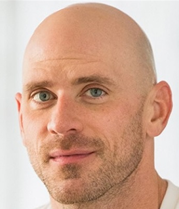
\includegraphics[width=0.2\textwidth]{face1.png}

\includegraphics[width=0.1\textwidth]{arrow.png}

\includegraphics[width=0.25\textwidth]{logo.png}

\includegraphics[width=0.1\textwidth]{arrow.png}
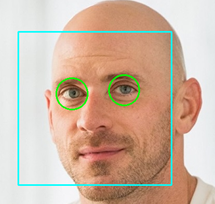
\includegraphics[width=0.25\textwidth]{face2.png}
\end{figure}
\end{frame}

\begin{frame}{Создание программы}
\begin{columns}
\column{0.6\textwidth}
\begin{itemize}
\item Для написания программы было решено воспользоваться библиотекой OpenCV и языком программирования C++
\item Библиотека уже содержит готовые каскады Хаара
\item Имея уже обученный каскад Хаара, можно вызывать функцию-обработчик, которая определяет наличие лица 
\item Чтобы наличие лица было явным, необходимо выделить его элементы: само лицо - в квадрат, а глаза - в круги
\end{itemize}
\column{0.5\textwidth}
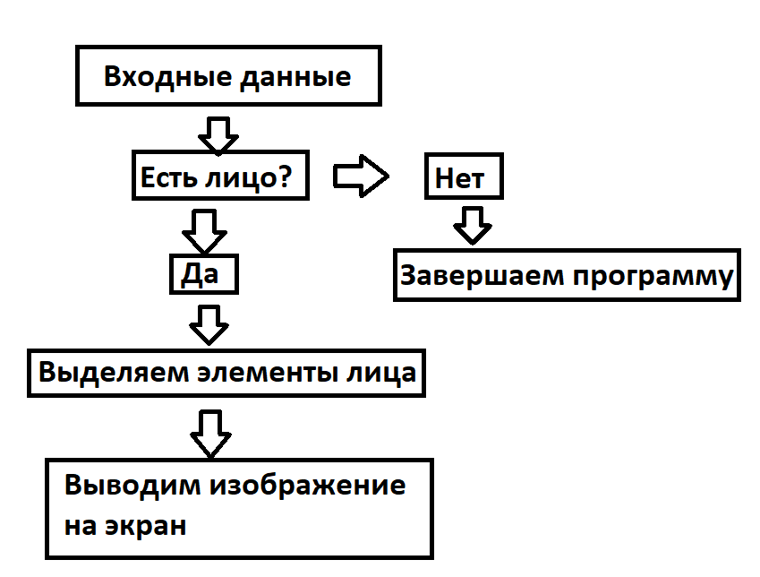
\includegraphics[width=1\textwidth]{algorythm.png}
\end{columns}
\end{frame}

\begin{frame}
\frametitle{Варианты работы программы}
 \begin{itemize}
 \item Изначально у пользователя есть выбор между 3 режимами анализа (анализ видео с веб-камеры, анализ изображения из файла или анализ видеозаписи из файла)
\item При выборе анализа файла пользователю предлагается выбрать желаемый файл через диалоговое окно, а при выборе анализа веб-камеры она открывается автоматически
 \end{itemize}
 \begin{figure}

\includegraphics[width=0.25\textwidth]{Camera.jpg}

\includegraphics[width=0.25\textwidth]{image.jpg}

\includegraphics[width=0.25\textwidth]{video.jpg}
 \end{figure}
\end{frame}


\begin{frame}[fragile]{Режим: анализ веб-камеры}
\begin{columns}
\column{0.5\textwidth}
\begin{figure}
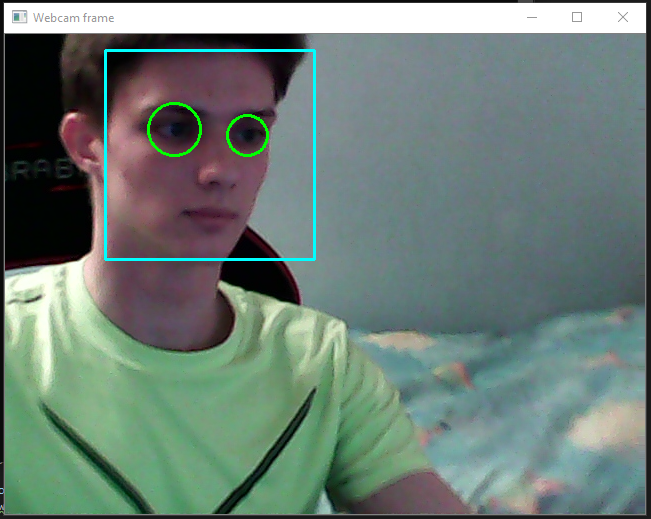
\includegraphics[width=1\textwidth]{cam1.png}
\end{figure}
\column{0.5\textwidth}
\begin{figure}
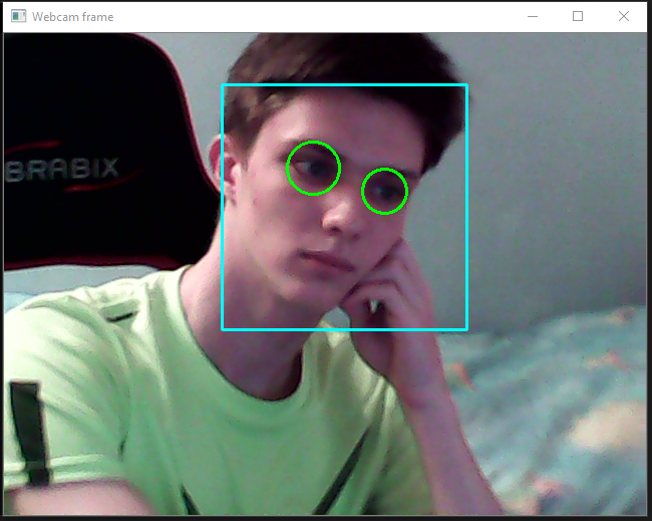
\includegraphics[width=1\textwidth]{cam2.png}
\end{figure}
\end{columns}
\end{frame}

\begin{frame}[fragile]{Режим: анализ изображения}
\begin{figure}
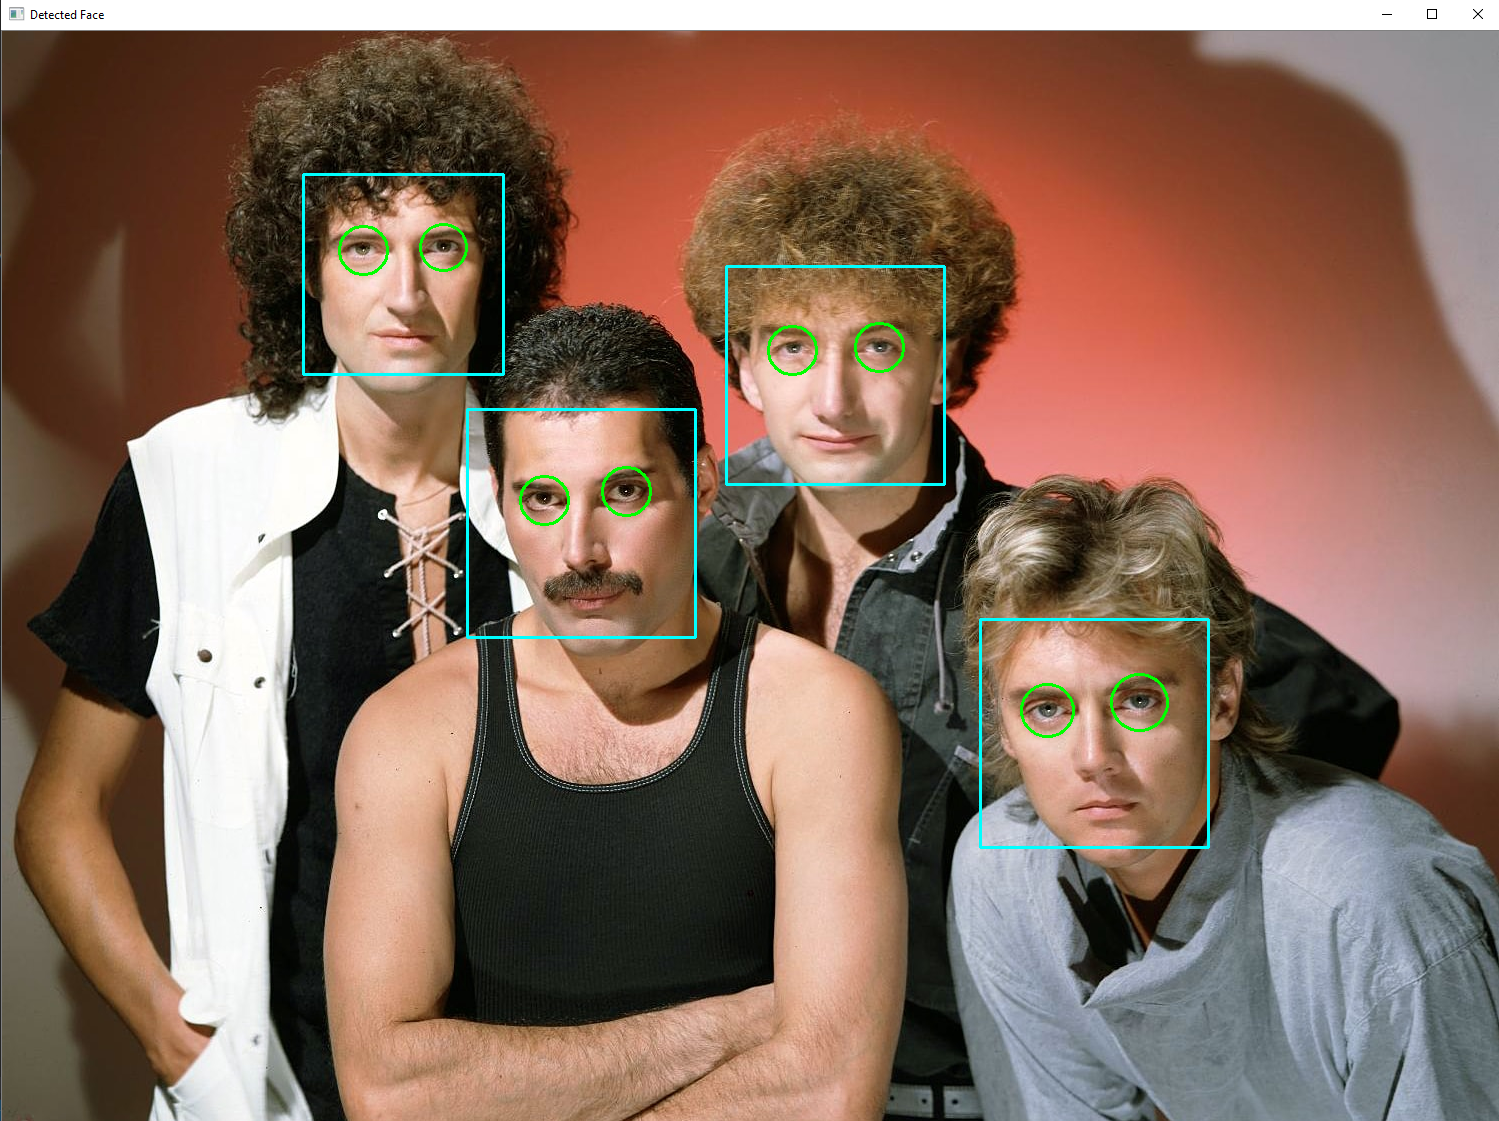
\includegraphics[width=0.9\textwidth]{image_ex.png}
\end{figure}
\end{frame}

\begin{frame}[fragile]{Режим: анализ видеофайла}
\begin{columns}
\column{0.5\textwidth}
\begin{figure}
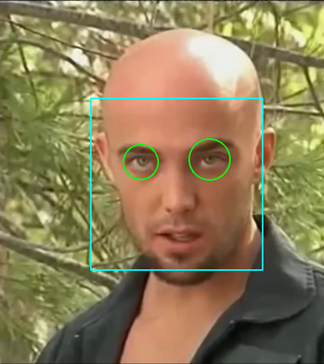
\includegraphics[width=0.9\textwidth]{vid1.png}
\end{figure}
\column{0.5\textwidth}
\begin{figure}
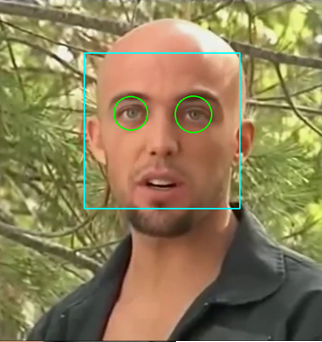
\includegraphics[width=0.9\textwidth]{vid2.png}
\end{figure}
\end{columns}
\end{frame}

\begin{frame}[fragile]{Заключение}
\begin{itemize}
\item Разработанная программа имеет 3 режима работы, что позволяет производить анализ практически любых цифровых файлов (или же видео в реальном времени)
\item Отличительной особенностью программы является тот факт, что алгоритмы обработки событий (какой анализ выбран) и функции обработчики никак не связаны с искомым объектом, то есть всего лишь заменив файла каскада Хаара на желаемый (например, вместо лица - автомобильный номер) можно получить приложение по распознаванию уже других объектов.
\end{itemize}
\end{frame}

\end{document}